% !TeX root = main.tex


\begin{savequote}[70mm]
,,Mapy mają dwie zasadnicze cechy: nie są terytorium, które opisują, ale, jeśli
są zrobione poprawnie, mają podobną do nich strukturę, co powoduje o ich
przydatnosci.''
\qauthor{Alfred Korzybski}
\end{savequote}


\chapter{System nawigacji}
\label{chap:mapa}

\section{Struktura systemu nawigacji}

Wybór struktury programowej ROS pociągnął za sobą w sposób naturalny kolejne
wybory związane ze strukturą systemu nawigacji robota. Zgodnie z filozofią
twórców tego oprogramowania, podsystem nawigacji dla robota mobilnego podzielony
jest na kilka modułów, których wzajemna współpraca i zależności pokazane są na
rysunku~\ref{fig:diag_move_base}. Część z nich jest dostarczana razem z systemem
ROS i wykorzystywana bez zmian w kodzie (of the shelf), niektóre mogą być
swobodnie wymieniane pod warunkiem, że spełniają wymogi odpowiednich interfejsów
(razem z systemem dostarczone są pewne implementacje, z których można
skorzystać), wymagane jest też dostarczenie kilku modułów zależnych od samego
robota, na którym całość jest uruchamiana.

\begin{figure}[h!]
\centering
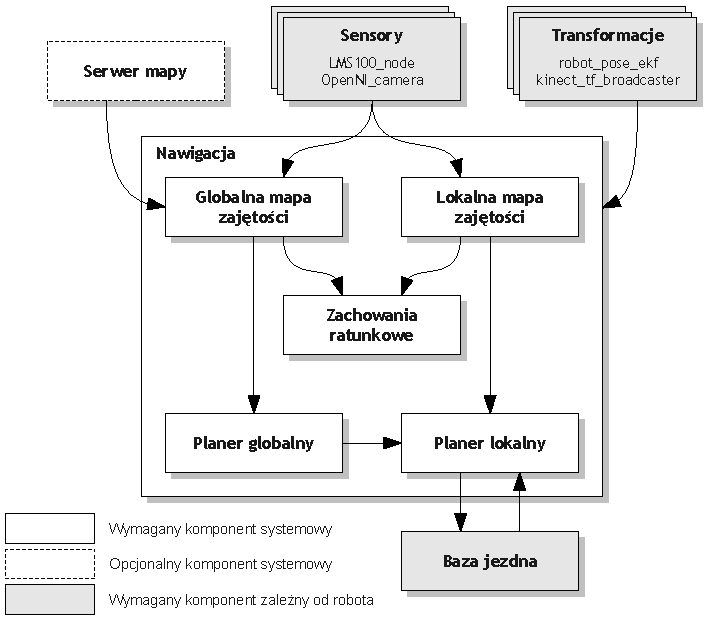
\includegraphics{../img/diag_move_base}
\caption{Struktura systemu nawigacji robota}
\label{fig:diag_move_base}
\end{figure}

Modułami, które są dostarczone i niezmienne są mapy przeszkód (konkretnie
moduły agregujące dane z sensorów i tworzące na ich podstawie mapy zajętości).
Modułami wymiennymi są planery trasy (zarówno lokalny jak i globalny) oraz
zachowania awaryjne mające na celu wyprowadzenie robota z trudnych sytuacji
(np. otoczenie przeszkodami). Dodatkowo wymagane jest dostarczenie przynajmniej
modułów sensorycznych, modułów określających lokalizację robota w pewnym,
globalnym układzie współrzędnych (może to być układ związany z punktem startowym
robota) oraz oczywiście głównego sterownika robota. Ogólnie cały system można
podzielić na trzy główne części, odpowiedzialne za wykrywanie przeszkód i
tworzenie lokalnych map zajętości (kosztu), lokalizację robota oraz planowanie
trasy (globalne i lokalne).

\section{Tworzenie map przeszkód}

Podczas poruszania się robota w środowisku o nie w pełni znanej strukturze
kluczowe jest wykrywanie aktualnej konfiguracji przeszkód. W środowiskach
statycznych wystarczy samo ich zaznaczanie na mapie, w przypadku otoczenia
dynamicznie się zmieniającego równie ważne jest wykrywanie momentów, w których
przeszkody znikają (czyszczenie przeszkód na mapie jest trudniejsze niż ich
oznaczanie). Cały proces wykrywania i oznaczania przeszkód można podzielić na
cztery etapy:

\begin{itemize}
  \item agregacja danych z sensorów,
  \item filtrowanie danych,
  \item oznaczanie przeszkód w pewnej, wybranej strukturze danych,
  \item tworzenie dwuwymiarowej mapy kosztu.
\end{itemize}

\subsection{Agregacja danych z czujników}

Pierwszym etapem jest zebranie danych z sensorów. W przypadku robota Elektron
istnieją dwa źródła danych o przeszkodach -- skaner laserowy SICK oraz sensor
Kinect. Biorąc pod uwagę wielkość otrzymywanych danych (w przypadku lasera
kilkaset punktów, w przypadku sensora Kinect kilka tysięcy na każdy pomiar) oraz
stosunkowo niewielką prędkość poruszania się robota, do wykrywania przeszkód
nie są wykorzystywane wszystkie odczyty, a jedynie pięć na sekundę w przypadku
lasera oraz dwa na sekundę w przypadku Kinecta. 

Po zebraniu pomiarów muszą one jeszcze zostać przetransformowane do wspólnego
układu współrzędnych, w tym przypadku do układu związanego z bazą robota (w
przypadku sensora Kinect należy także wziąć pod uwagę jego pochylenie względem
bazy). Za publikację wszystkich niezbędnych transformacji  odpowiedzialne są
komponenty \comp{kinect\_tf\_broadcaster} oraz \comp{laser\_tf}.

\subsection{Filtrowanie danych}

Dane odebrane z sensorów podlegają dalszemu procesowi filtracji, który ma na
celu usunięcie odczytów w jakikolwiek sposób zafałszowanych. Odczyty ze skanera
laserowego są obarczone takimi błędami w sposób niewielki, dlatego w tym
przypadku filtracja się nie odbywa. Inaczej przedstawia się kwestia odczytów z
Kinecta -- pojawiające się w nich pojedyncze, przypadkowe punkty mogą powodować
pojawianie się na mapie przeszkód uniemożliwiających ruch robota. Z tego powodu
stosowana jest filtracja danych ze względu na otoczenie punktów -- pojedyncze
odczyty, odstające od reszty pomiarów (posiadające w otoczeniu zbyt mało
sąsiadów) są odrzucane.

\subsection{Mapa wokselowa}

Wszystkie punkty, które przejdą przez proces filtracji, są przekazywane do
modułu tworzącego mapę zajętości. Wewnętrznie przechowuje on reprezentację
otoczenia w postaci mapy wokselowej (trójwymiarowa siatka prostopadłościanów).
Zmieniając wielkość oczek siatki możemy wybierać pomiędzy dokładnością pokrycia
otoczenia (im większe oczka, tym przeszkody będą zajmowały więcej miejsca, nawet małe
przeszkody będą reprezentowane przez całe zajęte oczka siatki) a szybkością
działania i obciążeniem systemu (małe oczka wymagają dużo większego nakładu
obliczeniowego). Implementacja dostępna w systemie ROS ze względów
optymalizacyjnych zakłada maksymalnie 16 poziomów siatki w pionie, nie jest to
jednak ograniczenie w sposób szczególny wpływające na jej uzyteczność. Dzięki
przyjętemu sposobowi reprezentacji (każda kolumna w mapie reprezentowana przy
pomocy jednej liczby całkowitej) można było natomiast zastosować wydajne
algorytmy śledzenia promieni (wykorzystywane przy czyszczeniu przeszkód z mapy).

Największym ograniczeniem tej struktury danych jest założenie, że robot porusza
się po płaskim terenie, na którym nie występują spadki (np. schody w dół), przez
co przeszkody o ,,ujemnej wysokości'' nie są w żaden sposób wykrywane. Niestety,
moduł odpowiedzialny za tworzenie map otoczenia nie jest przystosowany do
łatwego dostarczania własnych implementacji wewnętrznych struktur danych i
algorytmów (tak jak np. planery trasy). Istniały dwie możliwości
rozwiązania tego problemu: stworzenie kopii dużej części systemu i wprowadzanie
w niej własnych zmian, bądź napisanie modułu pośredniczącego pomiędzy sensorem a
algorytmami oznaczania przeszkód, która to metoda została wybrana.

\subsubsection{Oznaczanie przeszkód}

\subsubsection{Czyszczenie przeszkód}

\subsubsection{Wykrywanie spadków terenu}

\subsection{Mapa zajętości}

Po zaznaczeniu wszystkich przeszkód w mapie wokselowej, są one rzutowane na
dwuwymiarową mapę zajętości. Wszystkie kolumny, w których są oznaczone zajęte
komórki są oznaczane jako zajęte, jeśli natomiast w kolumnie są tylko komórki
puste bądź nieznane, to w zależności od ilości nieznanych oznaczenie jest rózne.
Jeśli więcej niż 4 komórki są nieznane, wtedy cała kolumna jest uznawana za
nieznaną, w przeciwnym wypadku kolumna jest uznawana za pustą.

Po oznaczeniu przeszkód dokonywane jest ich powiększenie na określoną odległość
(nadmuchiwanie). Operacja ta ma na celu wygładzenie mapy kosztu i spowodowanie,
że robot nie będzie preferował szerokie przejazdy (o ile będzie miał wybór). NA
rysunku~\ref{fig:inflation} przedstawiona jest ogólna metoda obliczania kosztu
dla komórki podczas tego procesu. Parametrem kontrolującym ten proces jest
promień ,,nadmuchiwania'', od którego zależy, jak dużą odległość od
przeszkód będzie zachowywał robot.

\begin{figure}[htb!]
\centering
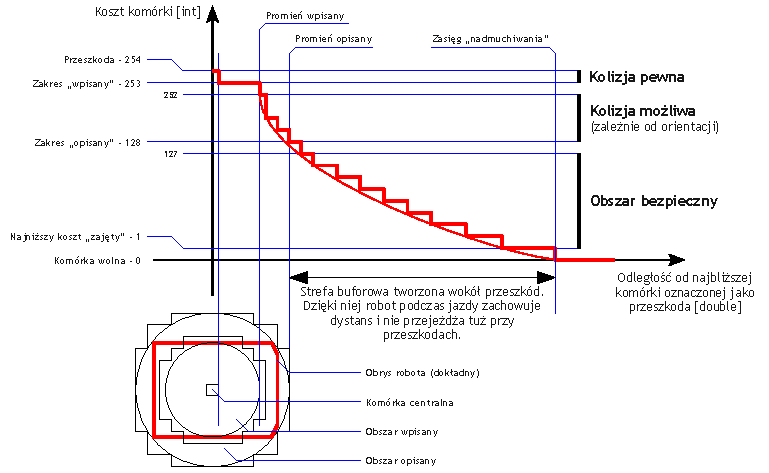
\includegraphics[width=15cm]{../../Common/img/ros/inflate.pdf}
\caption{Nadmuchiwanie przeszkód.}
\label{fig:inflation}
\end{figure} 

Mapa zajętości ma stały rozmiar, a jej środek związany jest ze środkiem bazy
jezdnej robota. W środowiskach o dynamicznie zmieniającej się konfiguracji
przeszkód przechowywanie globalnej mapy zajętości (innej niż statyczna mapa
otoczenia) często powoduje więcej problemów niż pożytku -- przeszkody widoczne
na niej w dużej odległości od robota mogą faktycznie już zniknąć, a pozostając
na mapie mogą zakłamywać globalne planowanie ścieżki. Dodatkowo wprowadzona jest
duża oszczędność pamięci, gdyż przechowywana mapa ma stały rozmiar, niezależnie
od przejechanego przez robota dystansu i wielkości eksplorowanego środowiska.

\section{Lokalizacja robota}


\section{Planowanie trasy}

\subsection{Ścieżka globalna}
\subsection{Ścieżka lokalna}
